\chapter{Strumenti numerici indicatori - parte IV}

\begin{figure}[h]
    \centering
    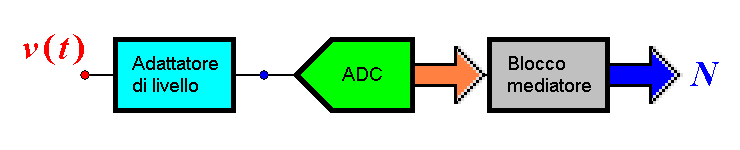
\includegraphics[scale = 1]{schema volmetro a valore medio schema usuale.png}
\end{figure}

\newpage    

\section{Voltmetro numerico a valore medio}
\footnote{Slide della prof | SDME 4 Strumenti numerici indicatori - parte IV | pag 2 \\  
Appunti | 2025-04-30 | pag 8 | 2025-05-06 | pag 2}

In questo capitolo ci concentreremo sull'architettura del voltmetro numerico a valore medio. \newline 

\begin{figure}[h]
    \centering
    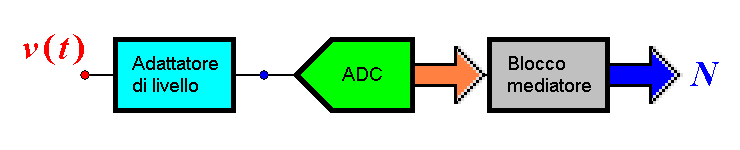
\includegraphics[scale = 1]{schema volmetro a valore medio schema usuale.png}
\end{figure}

In particolare a: 

\begin{itemize}
    \item partitore di ingresso 
    \item protezione contro le sovratensioni all'ingresso 
    \item convertitore AD a valore medio
\end{itemize}

Il voltmetro numerico a valor medio che studieremo è uno strumento che misura una tensione in continua DC. \newline 

\newpage 

\section{Voltmetro multi-portata per misurazioni in continua (valore medio) - schema di principio}
\footnote{Slide della prof | SDME 4 Strumenti numerici indicatori - parte IV | pag 3 \\  
Appunti | 2025-04-30 | pag 8 | 2025-05-06 | pag 2-3}

L'architettura di un voltmetro da così: 

\begin{figure}[h]
    \centering
    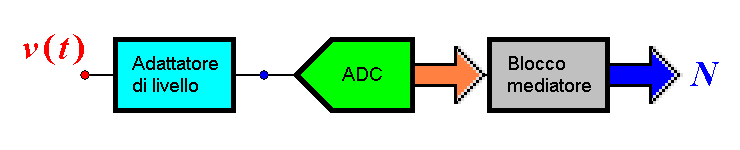
\includegraphics[scale = 1]{schema volmetro a valore medio schema usuale.png}
\end{figure}

passeremo a questa: 

\begin{figure}[h]
    \centering
    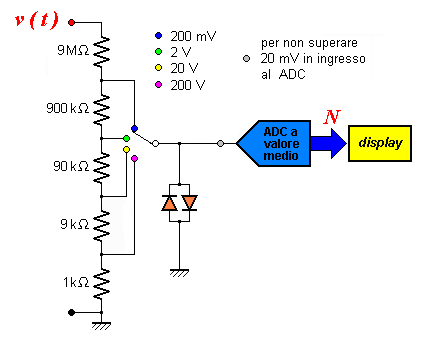
\includegraphics[scale = 2]{voltmetro numero con rete resistiva adattatore di livello.png}
\end{figure}

Quindi dal blocco adattatore di livello si passerà ad una rete resistiva, composta da 5 resistori. \newline 

Dalla figura, si può notare che questo tipo di architettura è di un voltmetro a 4 portate, rispettivamente 200 mV, 2 V, 20 V e 200 V, 
cioè si può impiegare lo stesso strumento, in questo caso il voltmetro, per tutti questi tipi di portate. \newline 

La portata del voltmetro va scelta in base all'intensità di picco del segnale v(t): 
per questo motivo è buona scelta, per avere incertezza minore, iniziare la misura con la portata maggiore e poi scendere fino alla portata ideale. \newline 

In base a dove si trova il selettore, la portata massima sarà quella che collega il pallino bianco a uno dei seguenti pallini: pallino blu scuro, verde, giallo, fucsia. \newline 

La rete resistiva ha una resistenza di: 

{
    \Large 
    \begin{equation}
        \begin{split}
        R_{in}
        &=
        9 \text{ } M \Omega
        + 
        900 \text{ } k \Omega
        + 
        90 \text{ } k \Omega
        + 
        9 \text{ } k \Omega
        + 
        1 \text{ } k \Omega
        \\
        &= 
        9 \text{ } \cdot 10^{6} 
        + 
        900 \text{ } \cdot 10^{3} 
        + 
        90 \text{ } \cdot 10^{3} 
        + 
        9 \text{ } \cdot 10^{3} 
        + 
        1 \text{ } \cdot 10^{3}
        [\Omega]
        \\
        &=
        10 \cdot 10^{6} [\Omega] 
        \\
        &= 
        10 \text{ } M \Omega
        \end{split}
    \end{equation}
}

La resistenza di ingresso: 

{
    \Large 
    \begin{equation}
        R_{in} = 10 \text{ M} \Omega
    \end{equation}
}

è un valore standard dei costruttore dei voltmetri. \newline 

Inoltre, come indicato nella figura dell'architettura, la tensione massima che deve andare all'ADC a valore medio (pallino grigio) 
non deve superare i 20 mV. \newline 

Per questo motivo, vengono scelti dei valori standard della rete resistiva e vengono posti due diodi in anti-parallelo per proteggere l'ADC da elevati correnti. \newline 

Idealmente l'ADC dovrebbe avere corrente nulla, in pratica può tollerare una corrente molto bassa. \newline   

Come ripetuto più volte in queste dispense, l'ADC è l'elemento più importante e costoso di uno strumento di misura: va trattato bene e con tante precauzioni. \newline 

\newpage 

\subsection{Adattatore di livello in ingresso (partitore di tensione)}
\footnote{Slide della prof | SDME 4 Strumenti numerici indicatori - parte IV | pag 4 \\  
Appunti | 2025-05-06 | pag 5 | 2025-06-23 Ricevimento | pag 6 - 7}

Il partitore di ingresso permette di adattare l'ampiezza del segnale al campo di misura consentito dal convertitore AD, che è di 20 mV. \newline 

Per minimizzare l'effetto dell'incertezza di quantizzazione, si deve impostare la portata immediatamente superiore al valore dell'incognita: 
ad esempio se v(t) è 1.5 V, è meglio impostare la portata del voltmetro a 2 V, non a 20 V. \newline 

Fisicamente, in un voltmetro, quello che si trova nello schema elettrico, lo possiamo visualizzare anche in questa maniera: 

\begin{figure}[h]
    \centering
    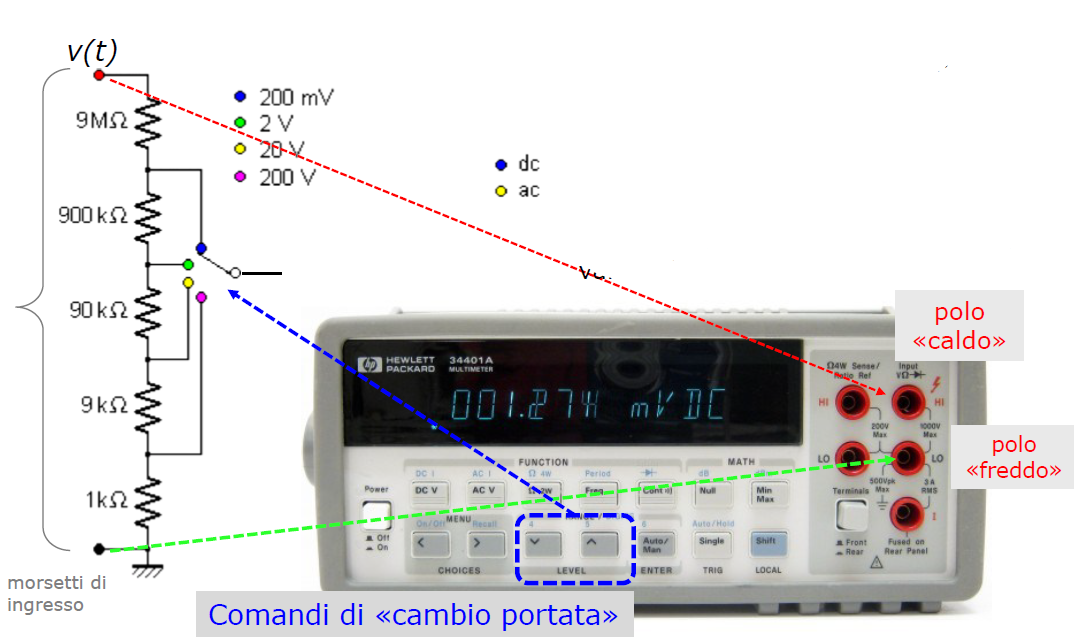
\includegraphics[scale = 0.8]{Da impostazioni voltmetro a rete resistiva.PNG}
\end{figure}

La figura ci dimostra come collegare i cavi per fare una misura e quali sono le implicazioni nell'adattatore di livello. \newline 

Il partitore è costituito da resistori di precisione e di elevata purezza, 
al fine di garantire la costanza dei rapporti di partizione, sia nel tempo che nella frequenza. \newline 

I resistori di precisione, essendo molto stabili in temperatura, in una rete resistiva, scelta una portata del voltmetro, 
manterranno stabile il rapporto di ripartizione della tensione di ingresso tra quella misurata ai capi del resistore rispetto alla rete resistiva totale. \newline 

Come scritto precedentemente, i resistori reali presentano una frequenza di taglio molto elevata rispetto alla frequenza dei segnali elettrici: 
ecco perchè in un voltmetro è anche indicato il range di frequenza in cui lo strumento opera. \newline 

Per rapporto di ripartizione costante nel tempo, si intende che i resistori di precisione "non invecchiano" con il tempo (o cambiano valore in diversi anni di utilizzo), 
quindi dopo diversi anni, il rapporto di ripartizione in una rete resistiva rimane costante. \newline 



\newpage 

\subsection{Dispositivi di protezione da sovraccarichi}
\footnote{Slide della prof | SDME 4 Strumenti numerici indicatori - parte IV | pag 5 \\  
Appunti | 2025-05-06 | pag 3} 

Dallo schema del voltmetro, notiamo che:

\begin{figure}[h]
    \centering
    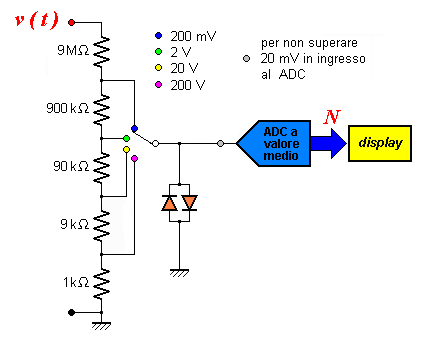
\includegraphics[scale = 2]{voltmetro numero con rete resistiva adattatore di livello.png}
\end{figure}

(da sinistra verso destra), dopo la rete resistiva e il selettore della portata massima, sono presenti due diodi in antiparallelo (quei due diodi arancioni in figura). \newline 

I due diodi in anti-parallelo proteggono i circuiti che seguono da tensioni troppo elevate; queste ultime potrebbero essere applicate per effetto di un uso errato dello strumento. \newline 

In questo caso, i due diodi in anti-parallelo proteggono l'ADC da tensioni maggiori di 20 mV, cioè abbassano la tensione elevata a 20 mV. \newline 




\newpage 

Idealmente, il diodo si comporta da interruttore dove, la relazione tra tensione ai capi del diodo e la corrente è la seguente: 

\begin{figure}[h]
    \centering
    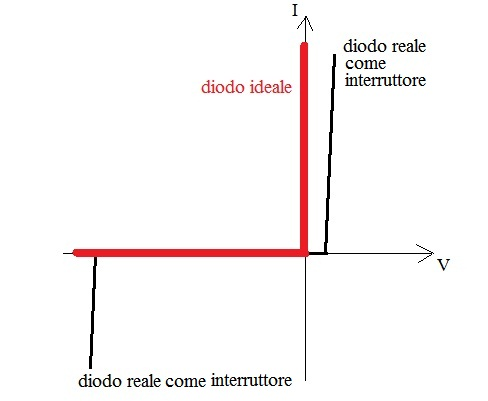
\includegraphics[scale = 0.5]{diodi18.jpg}
\end{figure}

Come visualizzato dalla seguente figura: 

\begin{figure}[h]
    \centering
    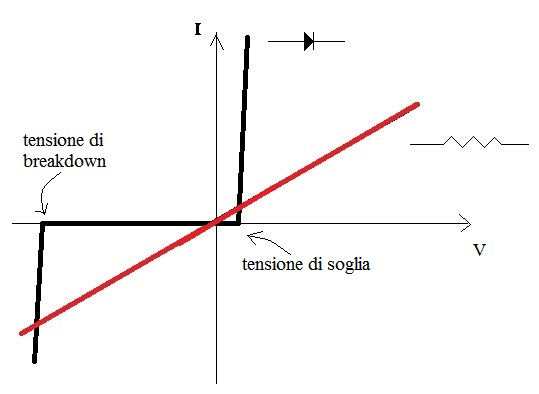
\includegraphics[scale = 0.5]{diodi17.jpg}
\end{figure}

si definisce tensione di soglia quando la curva di corrente del diodo diventa molto ripida. \newline 

Se la tensione ai capi del diodo è maggiore della tensione di bias, il diodo, idealmente, si comporta da interruttore chiuso. \newline 

Un'altra maniera di visualizzare il diodo: 

\begin{figure}[h]
    \centering
    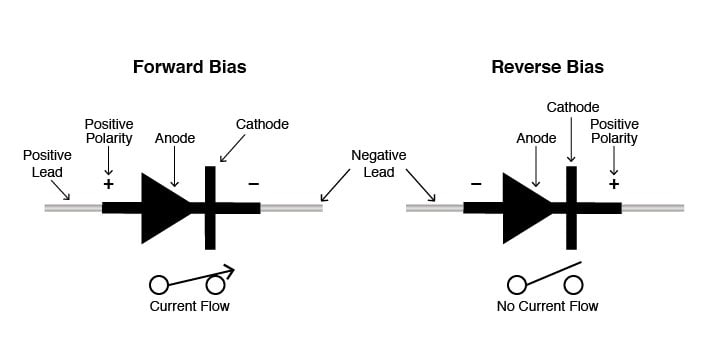
\includegraphics[scale = 0.5]{6004284b-dmm-how-to-diode-715x36.jpg}
\end{figure}

Visualizzando le curve tra tensione e corrente del diodo, si può notare che tensione e corrente sul diodo non hanno una relazione lineare, 
cioè non è una curva con pendenza costante (non è una curva $y = m \cdot x$): per questo motivo il diodo è un dispositivo non lineare. \newline 

Ritornando alla rete del voltmetro, quando lo strumento viene correttamente usato, la tensione applicata al dispositivo, in questo caso all'ADC, risulta non superiore a 20 mV. \newline

Quando la tensione di ingresso, proveniente dalla rete resistiva è maggiore di 20 mV, uno dei due diodi risulta "sotto soglia", mentre l'altro è polarizzato in inversa 
e la corrente derivata verso massa dai diodi è di valore trascurabile nei confronti della corrente che fluisce nel partitore di ingresso. \newline 

Il diodo in conduzione impone la tensione al nodo in comune con l'ADC la tensione massima di 20 mV e fa fluire tutte la corrente a massa. \newline 

Se la corrente è in direzione opposta, capiterà il caso opposto: sarà il diodo a sinistra in conduzione, quindi si comporterà da interruttore chiuso, mentre quello a destra non sarà in conduzione, 
quindi si comporterà da interruttore aperto. \newline 

Sapendo che i due diodi in antiparallelo impongono al nodo comune con il selettore e l'ADC la tensione massima di 20 mV, 
si può ritenere che il partitore di tensione (cioè la rete resistiva) operi a vuoto e che la tensione applicata ai circuiti di conversione sia una frazione nota dalla tensione incognita, 
cioè la tensione ai capi dei o del resistore scelto dal selettore. \newline 

Nel caso di sovraccarico, la tensione applicata ai blocchi di conversione può salire, fino a quando uno dei due diodi passa in "conduzione di potenza". \newline 

Quindi i diodi sono in conduzione se qualcosa non dovrebbe andare come previsto. \newline 

\newpage 

\subsection{Protezione contro sovratensioni}
\footnote{Slide della prof | SDME 4 Strumenti numerici indicatori - parte IV | pag 6-8 \\  
Appunti | 2025-05-06 | pag 3 - 5}

Riconsiderando il circuito del voltmetro, in particolare dei diodi in anti-parallelo: 

\begin{figure}[h]
    \centering
    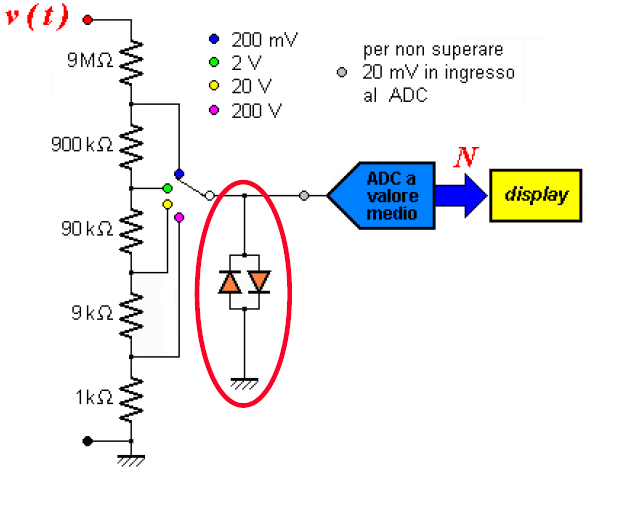
\includegraphics[scale = 1]{rete voltmetro con focus ai diodi in anti-parallelo.PNG}
\end{figure}

poniamo come esempio una tensione di 500 mV e una temperatura della giunzione a $25^{\circ}$ C. \newline 

\newpage 

Come visualizziamo dalla seguente figura  di un diodo di esempio in cui viene mostrata la relazione tra tensione ai capi sul diodo e la corrente che ci passa: 

\begin{figure}[h]
    \centering
    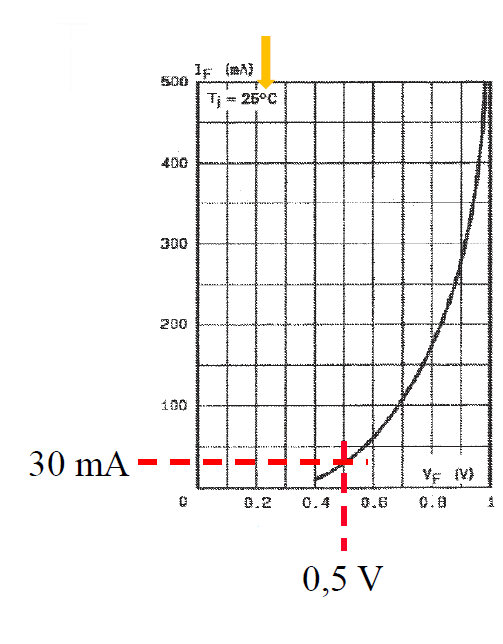
\includegraphics[scale = 1]{corrente di bias e tensione ai capi di un diodo di un volmetro.PNG}
\end{figure}

questo diodo, con una tensione ai capi di 500 mV, cioè 0.5 V, porta una corrente di 30 mA in polarizzazione diretta. \newline 

Tale corrente è trascurabile o meno? \newline 

Non lo è, rispetto alla corrente che circola sul partitore di tensione. \newline 

I diodi devono operare a bassissima tensione per limitare la corrente da essi derivata e occorre anche garantire che ci sia sempre almeno 
una resistenza del partitore inserita (in questo caso 9 M$\Omega$ ) per limitare la corrente che può circolare sui diodi ed evitare che si brucino. \newline 

Una volta che i diodi si bruciano, vanno immediatamente sostituiti: i costruttori li posizionano in un luogo ben visibile all'operatore e sono facilmente sostituibili. \newline 

Meglio sostituire dei diodi di protezione, che hanno un costo economico bassissimo, che un ADC. \newline 

Se consideriamo il caso in cui la tensione massima del voltmetro è di 200 V, la corrente massima che può circolare nel partitore è di: 

{
    \Large 
    \begin{equation}
        \begin{split}
            i_{\text{max partitore}}
            &= 
            \frac{v(t)}{R_{in}}
            \\
            &= 
            \frac{200 \text{ V}}{10 \text{ M}\Omega}
            \\
            &= 
            20 \text{ }\mu A
        \end{split}
    \end{equation}
}

Sapendo che la corrente lungo la rete resistiva non è nulla, non si può considerare la misura svolta dal voltmetro una misura a vuoto, 
ma è bassissima rispetto alle grandezze da misurare, quindi si considera nulla. \newline 

Ricordiamo che i diodi in anti-parallelo vengono posti in anti-parallelo perchè non sappiamo a priori la polarità di v(t). \newline 

Viene scelta come condizione la tensione massima di 20 mV all'ADC in modo che lo strumento non eroghi troppa corrente, perchè, idealmente, la corrente nel circuito dovrebbe essere nulla per svolgere una misura a vuoto. \newline 

Una regola ingegneristica è quella che il diodo deve proteggere l'ADC da correnti inferiori almeno 3 ordini di grandezza rispetto alla corrente massima sul partitore di tensione: 
ecco perchè occorrono tensioni di uscita del partitore molto basse. \newline 

\newpage 

\section{Resistenza di ingresso: perturbazione}
\footnote{Slide della prof | SDME 4 Strumenti numerici indicatori - parte IV | pag 9\\  
Appunti | 2025-05-06 | pag 5}

Come scritto nei capitoli precedenti, purtroppo, nella realtà, quando si fa una misura si va a perturbare il circuito sotto misura. \newline 

Se ci troviamo in questo banale esempio di misura della tensione di un generatore di tensione in DC: 

\begin{figure}[h]
    \centering
    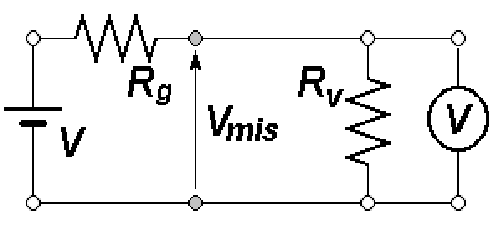
\includegraphics[scale = 1]{Perturbazione tensione misurata.png}
\end{figure}

Se si vuole misurare V, purtroppo si misurerà $V_{mis}$, che non è la tensione ai capi di V, bensì la tensione ai capi di $R_V$. \newline 

Possiamo considerare il seguente rapporto $\frac{\delta V}{V}$ la perturbazione, cioè il rapporto tra tensione misurata e tensione ai capi di V:

{
    \Large 
    \begin{equation}
        \frac{\delta V}{V} 
        = 
        - \frac{R_g}{R_g + R_v}
    \end{equation}
}

Il segno meno davanti al rapporto indica che la misura $V_{mis}$ è minore rispetto a V, quindi si sottostimerà V. \newline 

Per far tendere la perturbazione a zero, $R_g$ deve essere idealmente nulla, ma nella realtà molto piccola, 
invece $R_v$ deve essere idealmente infinita, nella realtà molto più grande di $R_g$, se possibile di diversi ordini di grandezza rispetto a $R_g$. \newline 

Ritornando alla rete resistiva del voltmetro: 

\begin{figure}[h]
    \centering
    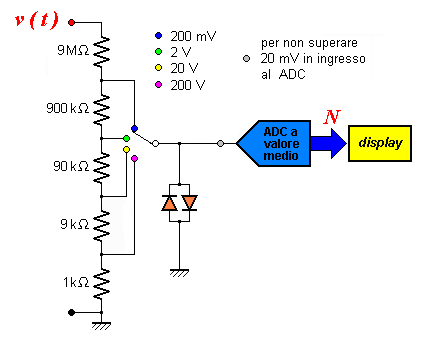
\includegraphics[scale = 1]{voltmetro numero con rete resistiva adattatore di livello.png}
\end{figure}

ecco perchè la somma dei resistori nell'adattatore di livello del voltmetro ha una resistenza pari a: 

{
    \Large 
    \begin{equation}
        R_v = 10 \text{ }M \Omega
    \end{equation}
}

perchè si considera $R_g$ sotto misura molto bassa, quindi la perturbazione della tensione sotto misura molto bassa. \newline 

\newpage 

\section{Convertitore AD a valor medio "tensione - tempo a doppia rampa"}
\footnote{Slide della prof | SDME 4 Strumenti numerici indicatori - parte IV | pag 10\\  
Appunti | 2025-05-06 | pag 6-7}

\begin{tcolorbox}
    Questo è l'argomento che chiede la prof più spesso all'esame, quindi lo dovete sapere come l'Ave Maria
\end{tcolorbox}

Di seguito l'architettura di un voltmetro: 

\begin{figure}[h]
    \centering
    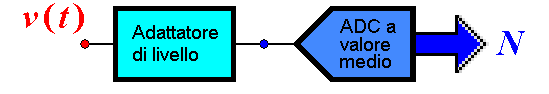
\includegraphics[scale = 1]{integrazione analogica voltmetro a valore medio.png}
\end{figure}

Ora che abbiamo studiato come è un adattatore di livello tipico all'interno di un voltmetro, passiamo all'altro elemento chiave: l'ADC a valor medio. \newline 

Ci possono essere e implementare diversi tipi di architetture di ADC: quello che andremo a spiegare sarà quello di un ADC a valor medio "tensione - tempo a doppia rampa". \newline 

Come è scritto nel nome dell'archietttura, si fa ricorso al tempo perchè, come scritto precedentemente, il tempo è la grandezza fisica che si può misurare con minor incertezza. \newline 

Si considera un ADC con incluso un riferimento di tensione $E_c$. \newline 

Di seguito lo schema di un convertitore AD a valor medio "tensione - tempo a doppia rampa": 

\begin{figure}[h]
    \centering
    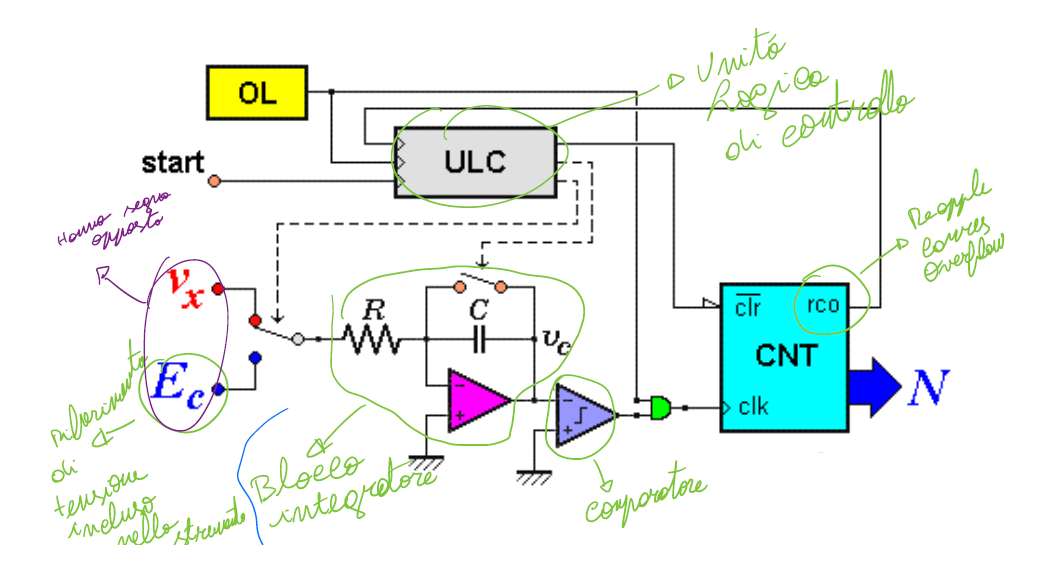
\includegraphics[scale = 0.85]{convertitore AD a valor medio tensione - tempo a doppia rampa con note.PNG}
\end{figure}

Come nel periodometro, intervallometro e frequenzimetro sono presenti l'oscillatore, il gate e il contatore (in figura OL rettangolo giallo, gate che è l'AND logico verde tra il comparatore e il contatore CNT, e il CNT contatore, il blocco azzurrino). \newline 

L'ULC (blocco grigio) governa il funzionamento dell'ADC. \newline 

$V_x$ è la tensione sotto misura. \newline 

$E_c$ è il riferimento di tensione dello strumento, che è di polarità opposta rispetto a $V_x$. \newline 

Tra $V_x$ e la resistenza R è presente un selettore, che sarà gestito dall'ULC. \newline 

La configurazione R resistore, C condensatore e Amplificatore operazione AmpOp (in figura triangolo di colore fucsia) 
possiamo considerarlo come blocco integratore. \newline 

\begin{tcolorbox}
    Per ripassare al volo perchè la configurazione RC con OpAmp è un blocco integratore, puoi visualizzare i seguenti link: 
    \begin{itemize}
        \item Amplificatore operazionale integratore by Edutecnica \\ \url{https://www.edutecnica.it/elettronica/id/id.htm} 
        \item Op-Amp Integrator (with Derivation and Solved Examples) by ALL ABOUT ELECTRONICS \\ \url{https://youtu.be/OPvs7A554Rw?si=26UEyYRwTgAwH3e9}
    \end{itemize}
\end{tcolorbox}

\newpage 

\subsection{Funzionamento ideale}
\footnote{Slide della prof | SDME 4 Strumenti numerici indicatori - parte IV | pag 11 - 15\\  
Appunti | 2025-05-06 | pag 7 - 9}

Di seguito lo schema di un convertitore AD a valor medio "tensione - tempo a doppia rampa": 

\begin{figure}[h]
    \centering
    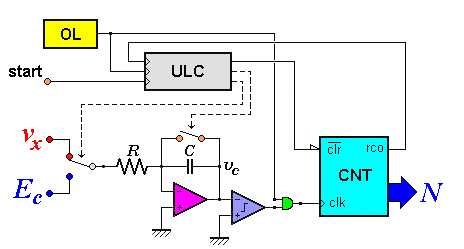
\includegraphics[scale = 1.5]{convertitore AD a valor medio tensione - tempo a doppia rampa.PNG}
\end{figure}

Di seguito saranno mostrate le linee dei pin. \newline 

La misura non inizia se il livello logico della linea di start non è alto: 

\begin{figure}[h]
    \centering
    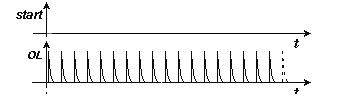
\includegraphics[scale = 1.5]{funzionamento ideale parte 1 ADC a valor medio.png}
\end{figure}

L'OL oscillatore locale manda i suoi segnali in modo continuo. \newline 

\newpage 

Al tempo $t_0$, gli andamenti dei pin nel circuito sono i seguenti: 

\begin{figure}[h]
    \centering
    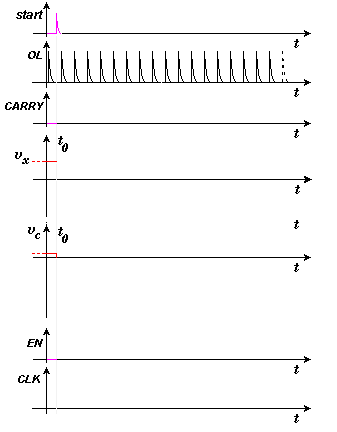
\includegraphics[scale = 1]{funzionamento ideale parte 2 ADC a valor medio.png}
\end{figure}

Al tempo $t_0$, il segnale di start diventa alto. \newline 

Quindi si resetta il resto del contatore CNT (nell'andamento dei pin è indicato con la scritta CARRY, nella figura dell'architettura è il pin rco del CNT). \newline 

Inoltre, la tensione $v_c$, cioè la tensione in comune all'AmpOp e il condensatore C si riporta a zero perchè l'ULC abbassa l'interruttore del circuito integratore: 

\begin{figure}[h]
    \centering
    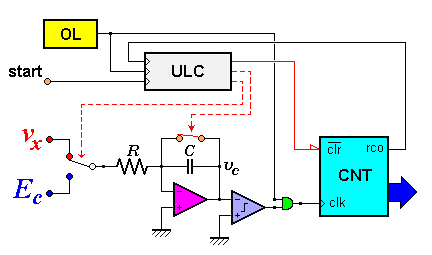
\includegraphics[scale = 1]{convertitore AD a valor medio tensione - tempo a doppia rampa interruttore chiuso.PNG}
\end{figure}

In questo modo, al tempo $t_0$ idealmente, il condensatore si scarica e si resetta istantaneamente. \newline 

In pin di EN (Enable) è il pin che si trova all'uscita del comparatore (triangolo violetto), 
uno dei pin di ingresso del gate AND. \newline 

Idealmente, tutti il CARRY e il condensatore C si resettano in modo istantaneo nel tempo $t_0$. \newline 

Ora che è tutto resettato, si procede alla misura della tensione di ingresso $v_x$. \newline 

\newpage 

L'interruttore viene subito riportato a livello alto: 

\begin{figure}[h]
    \centering
    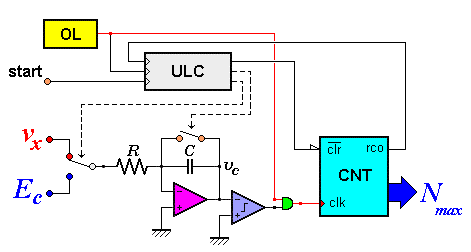
\includegraphics[scale = 1]{convertitore AD a valor medio tensione - tempo a doppia rampa interruttore aperto dopo reset.PNG}
\end{figure}

Definiamo ora un altro di istante di tempo $t_0$ in cui si ha il primo fronte d'onda dell'oscillatore locale OL a seguito del segnale logico alto di start: 
l'istnte $t_0$ è l'istante in cui inizia la misura. \newline 

L'andamento dei pin nel circuito sarà  il seguente: 

\begin{figure}[h]
    \centering
    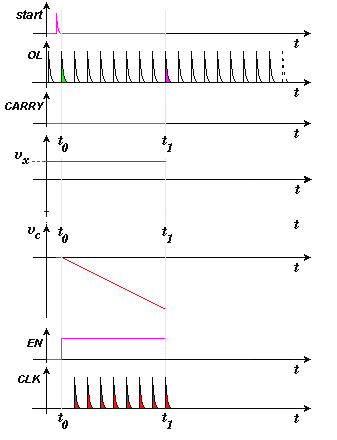
\includegraphics[scale = 1]{funzionamento ideale parte 3 ADC a valor medio.png}
\end{figure}

Come nel caso del periodometro, vengono contati quanti impulsi di clock dell'OL ci sono stati nel periodo tra $t_0$ e $t_1$, cioè finché il bit di CARRY del CNT è basso. \newline 

Come si vede dall'andamento della tensione $v_c$, 
la tensione $v_x$, passando per il blocco integratore, viene invertita di polarità perchè l'AmpOp è in configurazione invertente (il nodo positivo è collegato a massa, il nodo negativo è collegato al nodo con R e C). \newline 

\begin{tcolorbox}
    Altro ripasso di elementi di elettronica al volo: \\
    TENSIONE DI USCITA DI UN AMPLIFICATORE INVERTENTE by CorsiConsulenze NPR \\
    \url{https://www.youtube.com/watch?v=npqMyVCP-4o}
\end{tcolorbox}

Essendo un blocco integratore, l'integrale di una funzione costante è una retta con pendenza costante: 
in questo caso di pendenza negativa perchè l'AmpOp è configurazione inversa. \newline 

Il comparatore ha nel pin negativo proprio la tensione $v_c$: 
la tensione nel pin positivo è collegato a massa (cioè tensione nulla), quindi, essendo la tensione di massa maggiore di $v_c$, 
il comparatore dà come uscita un livello alto logico (vedi andamento del pin EN). \newline 

Come si può visualizzare dall'andamento del pin di CLK, che è un pin di ingresso del contatore CNT, 
essendo il gate un AND logico, se il pin EN è alto e il pin OL è alto, allora il pin clk avrà un livello alto. \newline  

Tra il tempo $t_0$ e $t_1$ il CNT conterà i fronti di salita del clock in quel periodo. \newline 

Al tempo $t_1$ il CNT raggiunge la sua capienza massima ed eroga il suo $N_{max}$, che vale: 

{
    \Large 
    \begin{equation}
        N_{max} = 2^{n} - 1
    \end{equation}
}

dove n è il numero di bit del CNT. \newline 

Per questo motivo, il CNT si resetta a zero e il pin di CARRY diventa alto, 
come visualizzato dalle seguenti figura: 

\begin{figure}[h]
    \centering
    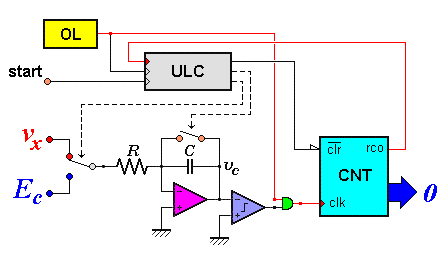
\includegraphics[scale = 1]{convertitore AD a valor medio tensione - tempo a doppia rampa CNT overflow.PNG}
    \\
    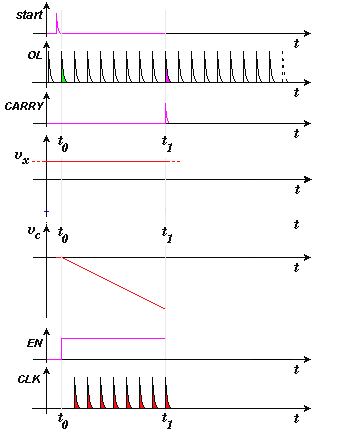
\includegraphics[scale = 1]{funzionamento ideale parte 4 ADC a valor medio.png}
\end{figure}

A questo punto l'ULC cambia il selettore, da $v_x$ a $E_c$: 

\begin{figure}[h]
    \centering
    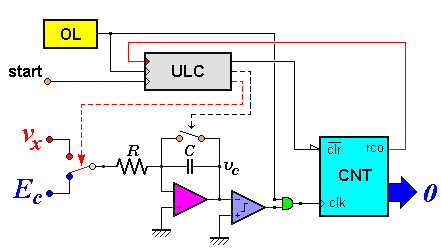
\includegraphics[scale = 1]{convertitore AD a valor medio tensione - tempo a doppia rampa Ec selettore.PNG}
\end{figure}

\newpage 

L'andamento dei pin, all'istante $t_1$, sarà il seguente: 

\begin{figure}[h]
    \centering
    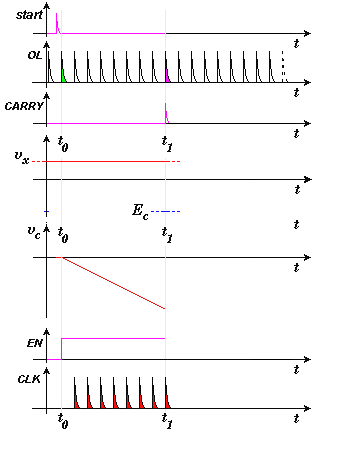
\includegraphics[scale = 1]{funzionamento ideale parte 5 ADC a valor medio.png}
\end{figure}

L'andamento dei pin, dall'istante $t_1$ in poi, sarà il seguente: 

\begin{figure}[h]
    \centering
    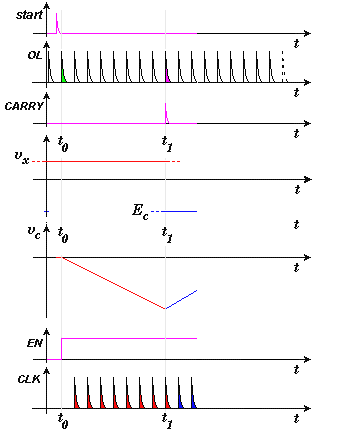
\includegraphics[scale = 1]{funzionamento ideale parte 6 ADC a valor medio.png}
\end{figure}

Visualizzando l'andamento della tensione $v_c$, la pendenza della curva di tensione è diversa prima e dopo l'istante $t_1$ 
(nella figura pendenza curva rossa e curva blu diversa). \newline 

\newpage 

Il circuito andrà avanti finché $v_c$ sarà uguale a zero: 

\begin{figure}[h]
    \centering
    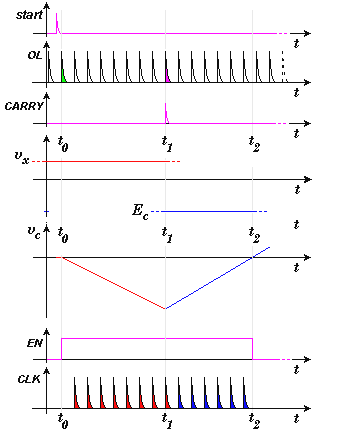
\includegraphics[scale = 1]{funzionamento ideale parte 7 ADC a valor medio.png}
\end{figure}

A questo punto, la misura di $v_x$ è finita. \newline 

Quello che a noi interessa, sono gli impulsi di clock dell'OL dall'istante $t_1$ all'istante $t_2$ (gli impulsi di colore blu nell'andamento del pin CLK), 
cioè quando $v_c = 0$. \newline 

Con questo tipo di architettura, è possibile determinare la tensione media di $v_x$ tra il tempo [$t_0$, $t_1$] come: 

{
    \Large 
    \begin{equation}
        \left.
        \overline{v_x}
        \right|_{[t_0, t_1]}
        = 
        - E_c 
        \frac{N}{N_{max}}
    \end{equation}
}

L'intervallo di tempo tra [$t_0$, $t_1$] è noto a priori, a differenza dell'intervallo [$t_1$, $t_2$]. \newline 

Sappiamo che: 

{
    \Large 
    \begin{equation}
        \abs{t_0 - t_1} = N_{max} \cdot \tau
    \end{equation}
}

dove $\tau$ è la durata dell'impulso dell'OL. \newline 

Invece non conosciamo a priori l'intervallo $\abs{t_1 - t_2}$. \newline 

Ma sappiamo che, sicuramente: 

{
    \Large 
    \begin{equation}
        \abs{t_0 - t_1} 
        <
        \abs{t_1 - t_2}
    \end{equation}
}

perchè il CNT, nel periodo [$t_1$, $t_2$], non arriva a $N_{max}$. \newline 

\newpage 

\subsection{Analisi funzionamento ideale}
\footnote{Slide della prof | SDME 4 Strumenti numerici indicatori - parte IV | pag 16 - 17\\  
Appunti | 2025-05-07 | pag 2}

Adesso concentriamoci sull'analisi dell'andamento delle tensioni di $v_x$, la tensione sotto misura, e $v_c$, la tensione dopo il blocco integratore: 

\begin{figure}[h]
    \centering
    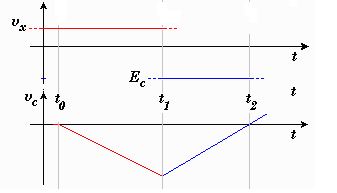
\includegraphics[scale = 2]{Andamento di vx e vc in un ADC a valor medio.png}
\end{figure}

All'istante $t_0$, la tensione $v_c$ possiamo scriverla come:

{
    \Large 
    \begin{equation}
        v_c(t_0) = 0
    \end{equation}
}

All'istante $t_1$, la tensione $v_c$ sarà: 

{
    \Large 
    \begin{equation}
        v_c(t_1) = v_c(t_0) + \int_{t_0}^{t_1} \frac{v_x(t)}{-RC} dt
    \end{equation}
}

dove $\int_{t_0}^{t_1} \frac{v_x(t)}{-RC}$ è dovuto al blocco integratore RC con AmpOp invertente dell'ADC. \newline 

\begin{tcolorbox}
    In analisi matematica 1 (mitico Montecchiari), abbiamo studiato che un'integrale definito possiamo scriverlo come: 

    {
        \Large 
        \begin{equation}
            \begin{split}
            \int_{a}^{b} f(x) dx
            &=
            \left.
            F(x)
            \right|_{a}^{b} + c
            \\
            &=
            F(a) - F(b) + c
            \end{split}
        \end{equation}
    }

    dove F(a) è la primitiva di f(x) nel punto a, F(b) è la primitiva di f(x) nel punto b e +c è la costante di integrazione. \newline 

    In questo caso gli estremi di integrazione sono $t_1$ e $t_0$, la funzione è $\frac{v_x(t)}{-RC}$ 
    e la costante di integrazione è $v_c(t_0)$. 
\end{tcolorbox}

All'istante $t_2$ la tensione $v_c$ sarà uguale a:

{
    \Large 
    \begin{equation}
        v_c(t_2)
        = 
        v_c(t_1)
        + 
        \int_{t_1}^{t_2} \frac{E_c (t)}{-RC} dt   
    \end{equation}
}

Nella frazione dell'integrale è presente $E_c (t)$ al posto di $v_x (t)$ perchè all'istante $t_1$, 
l'ULC ha cambiato il selettore da $v_x(t)$ a $E_c(t)$. \newline 

Sapendo che all'instante $t_2$, $v_c$ vale: 

{
    \Large 
    \begin{equation}
        v_c(t_2) = 0
    \end{equation}
}

possiamo scrivere: 

{
    \Large 
    \begin{equation}
        \begin{split}
            v_c(t_2) 
            &=
            v_c(t_1)
            + 
            \int_{t_1}^{t_2} \frac{E_c (t)}{-RC} dt
            \\ 
            &= 
            v_c(t_0) + \int_{t_0}^{t_1} \frac{v_x(t)}{-RC} dt + \int_{t_1}^{t_2} \frac{E_c (t)}{-RC} dt
            \\
            &= 
            0
        \end{split}
    \end{equation}
}

Sapendo i valori di $v_c$ agli instanti $t_0$ e $t_2$ e compiendo dei semplici passaggi algebrici, 
la scorsa equazione diventa:

{
    \Large 
    \begin{equation}
        \begin{split}
            v_c(t_2) 
            &=
            v_c(t_0) + \int_{t_0}^{t_1} \frac{v_x(t)}{-RC} dt + \int_{t_1}^{t_2} \frac{E_c (t)}{-RC} dt
            \\
            &\downarrow
            \\
            0
            &= 
            0 + \int_{t_0}^{t_1} \frac{v_x(t)}{-RC} dt + \int_{t_1}^{t_2} \frac{E_c (t)}{-RC} dt
            \\
            - \int_{t_0}^{t_1} \frac{v_x(t)}{-RC} dt 
            &=
            \int_{t_1}^{t_2} \frac{E_c (t)}{-RC} dt
            \\
            \int_{t_0}^{t_1} \frac{v_x(t)}{RC} dt 
            &=
            \int_{t_1}^{t_2} \frac{E_c (t)}{-RC} dt
        \end{split} 
    \end{equation}
}

Quindi, l'equazione finale da risolvere e da analizzare è la seguente: 

{
    \Large 
    \begin{equation}
        \int_{t_0}^{t_1} \frac{v_x(t)}{RC} dt 
        =
        \int_{t_1}^{t_2} \frac{E_c (t)}{-RC} dt
    \end{equation}
}

\newpage 

\subsection{Primo vincolo sulla stabilità}
\footnote{Slide della prof | SDME 4 Strumenti numerici indicatori - parte IV | pag 18\\  
Appunti | 2025-05-07 | pag 2}

\begin{tcolorbox}
    Come detto a lezione dalla prof, la matematica per un ingegnere non è il fine ma un mezzo: ecco perchè vanno fatte queste osservazioni riguardo alla stabilità. \newline

    La matematica descrive il mondo fisico, ma non è il mondo fisico. \newline 
\end{tcolorbox}

L'equazione da analizzare è la seguente: 

{
    \Large 
    \begin{equation}
        \int_{t_0}^{t_1} \frac{v_x(t)}{RC} dt 
        =
        \int_{t_1}^{t_2} \frac{E_c (t)}{-RC} dt
    \end{equation}
}

Se i valori del resistore R e del condensatore C sono stabili, quindi mantengono il loro valore noto nell'intervallo $[t_0, t_2]$ 
perchè la temperatura è costante, i componenti fisici sono componenti di precisione e l'intervallo $[t_0, t_2]$ non è così elevato da modificare i valori di R e C, 
allora possiamo portare fuori dagli integrali la costante $\frac{1}{RC}$ e semplificare l'equazione come: 

{
    \Large 
    \begin{equation}
        \begin{split}
        \int_{t_0}^{t_1} \frac{v_x(t)}{RC} dt 
        &=
        \int_{t_1}^{t_2} \frac{E_c (t)}{-RC} dt
        \\
        &\downarrow
        \\
        \frac{1}{RC}
        \int_{t_0}^{t_1} v_x(t) dt 
        &=
        \frac{-1}{RC}
        \int_{t_1}^{t_2} E_c (t) dt
        \\
        \int_{t_0}^{t_1} v_x(t) dt 
        &=
        -
        \int_{t_1}^{t_2} E_c (t) dt
    \end{split}
    \end{equation}
}

Il valore del condensatore C, generalmente, non varia in base alla temperatura, bensì ciò che influisce di più nell'ambiente è l'umidità, 
perchè quest'ultima, varia la costante dielettrica $\varepsilon_r$ del condensatore C. \newline 

Quindi, dopo il primo vincolo sulla stabilità, 
l'equazione nell'ADC tensione a valor medio tempo a doppia rampa diventa:

{
    \Large 
    \begin{equation}
        \int_{t_0}^{t_1} v_x(t) dt 
        =
        -
        \int_{t_1}^{t_2} E_c (t) dt
    \end{equation}
}


\newpage 

\subsection{Secondo vincolo sulla stabilità}
\footnote{Slide della prof | SDME 4 Strumenti numerici indicatori - parte IV | pag 19\\  
Appunti | 2025-05-07 | pag 3}

Dopo il primo vincolo sulla stabilità, l'equazione da analizzare è: 

{
    \Large 
    \begin{equation}
        \int_{t_0}^{t_1} v_x(t) dt 
        =
        -
        \int_{t_1}^{t_2} E_c (t) dt
    \end{equation}
}

Sapendo che $E_c(t)$ è il riferimento di tensione nell'ADC e che è costante nell'intervallo $[t_1, t_2]$ e che quindi $E_c$ non dipende dal tempo t, 
allora l'equazione diventa: 

{
    \Large 
    \begin{equation}
        \begin{split}
        \int_{t_0}^{t_1} v_x(t) dt 
        &=
        -
        \int_{t_1}^{t_2} E_c (t) dt
        \\
        &\downarrow
        \\
        \int_{t_0}^{t_1} v_x(t) dt 
        &=
        -
        \int_{t_1}^{t_2} E_c dt
        \\
        \int_{t_0}^{t_1} v_x(t) dt 
        &=
        - E_c
        \int_{t_1}^{t_2}  dt
        \\
        &= 
        -E_c (t_2 - t_1)
        \end{split}
    \end{equation}
}

Siccome il nostro obbiettivo è calcolare la media di $v_x(t)$ nell'intervallo $[t_0, t_1]$, 
grazie al teorema della media integrale studiato ad Analisi Matematica 1, l'equazione diventerà:

{
    \Large 
    \begin{equation}
        \begin{split}
          \int_{t_0}^{t_1} v_x(t) dt 
        &=  
        -E_c (t_2 - t_1)
        \\
        &\downarrow
        \\
        \frac{1}{t_1 - t_0}
        \int_{t_0}^{t_1} v_x(t) dt 
        &=  
        \frac{1}{t_1 - t_0}
        \left[
        -E_c (t_2 - t_1)
        \right]
        \\
        &=  
        -E_c 
        \frac{t_2 - t_1}{t_1 - t_0}
        \end{split}
    \end{equation}
}

Quindi, dopo il secondo vincolo sulla stabilità, 
l'equazione nell'ADC a valor medio tensione tempo a doppia rampa diventa:

{
    \Large
    \begin{equation}
       \frac{1}{t_1 - t_0}
        \int_{t_0}^{t_1} v_x(t) dt 
        =   
        -E_c 
        \frac{t_2 - t_1}{t_1 - t_0}
    \end{equation}
}

\newpage 

\subsection{Espressione finale}
\footnote{Slide della prof | SDME 4 Strumenti numerici indicatori - parte IV | pag 20\\  
Appunti | 2025-05-07 | pag 4-5}

L'equazione da analizzare è la seguente: 

{
    \Large
    \begin{equation}
       \frac{1}{t_1 - t_0}
        \int_{t_0}^{t_1} v_x(t) dt 
        =   
        -E_c 
        \frac{t_2 - t_1}{t_1 - t_0}
    \end{equation}
}

Dopo aver spiegato il funzionamento dell'ADC e sapendo che è presente nell'architettura un OL-GATE-CNT, 
sappiamo che gli intervalli $t_1 - t_0$ e $t_2 - t_1$ sono uguali a: 

{
    \Large 
    \begin{equation}
        \begin{cases}
            t_1 - t_0 = N_{max} \cdot \tau 
            \\
            t_2 - t_1 = N \cdot \tau
        \end{cases}
    \end{equation}
}

dove $\tau$ è il tempo di un OL, $N_{max}$ è la capienza massima del CNT, e N sono il numero di impulsi dell'OL che vogliamo contare per misurare $\left. \overline{v_x} \right|_{[t_0, t_1]}$. \newline 

Grazie a queste considerazioni, possiamo semplificare l'equazione dell'ADC a valor medio tensione tempo a doppia rampa così: 

{
    \Large 
    \begin{equation}
        \begin{split}
        \frac{1}{t_1 - t_0}
        \int_{t_0}^{t_1} v_x(t) dt 
        &=   
        -E_c 
        \frac{t_2 - t_1}{t_1 - t_0}
        \\
        &\downarrow
        \\  
        \left. \overline{v_x} \right|_{[t_0, t_1]}
        &\approx 
        -E_c 
        \frac{N \tau}{N_{max} \tau}
        \end{split}
    \end{equation}
}

Questa ultima espressione ci dice che, per calcolare il valore di $\left. \overline{v_x} \right|_{[t_0, t_1]}$ abbiamo due gradi di libertà: 
\begin{itemize}
    \item o avere un $\tau$ molto breve, quindi un OL molto veloce 
    \item o avere un CNT molto grande, quindi un registro del contatore molto elevato
\end{itemize}

Continuando con le semplificazioni: 

{
    \Large 
    \begin{equation}
        \begin{split}
        \left. \overline{v_x} \right|_{[t_0, t_1]}
        &\approx 
        -E_c 
        \frac{N \tau}{N_{max} \tau}
        \\
        &= 
        -E_c 
        \frac{N }{N_{max}}
        \\
        &= 
        \frac{-E_c}{N_{max}} N
        \end{split}
    \end{equation}
}

Si è semplificato il $\tau$ nella espressione perchè il tempo di $\tau$ è lo stesso (l'OL nell'ADC di N e $N_{max}$ è lo stesso). \newline 

Si è posto nell'espressione il segno circa $\approx$ per i problemi di sincronizzazione che abbiamo precedentemente descritto nell'intervallometro, frequenzimetro e periodometro. \newline 

\newpage 

Per concludere, dall'architettura dell'ADC a valor medio tensione - tempo doppia-rampa 

\begin{figure}[h]
    \centering
    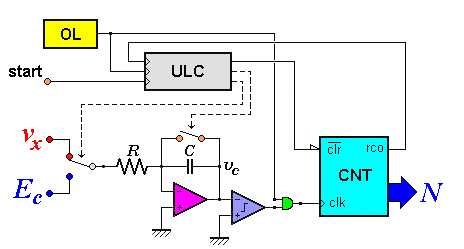
\includegraphics[scale = 1]{convertitore AD a valor medio tensione - tempo a doppia rampa.PNG}
\end{figure}


la tensione media di $v_x$ nell'intervallo $[t_0, t_1]$ sarà uguale a: 

{
    \Large 
    \begin{equation}
    \left. \overline{v_x} \right|_{[t_0, t_1]}
    \approx  
    \frac{-E_c}{N_{max}} N
    \end{equation}
}

Ricordiamo che la misura non inizia dal segnale alto di start, 
bensì dal segnale alto del pin EN del gate, che coincide con un fronte di salita dell'OL dopo l'istante del segnale alto di start. \newline 

\newpage

\subsection{Scelta dell'intervallo $[t_0, t_1]$ di integrazione}
\footnote{Slide della prof | SDME 4 Strumenti numerici indicatori - parte IV | pag 21\\  
Appunti | 2025-05-07 | pag 5}

Anche la scelta dell'intervallo di tempo è molto importante. \newline 

Come descritto nei capitoli precedenti, sapendo che, a causa del residuo di rete della rete di distribuzione elettrica in Europa e in America, 
si sceglie una finestra di misurazione di 100 ms perchè è 5 volte il tempo di disturbo della rete europea e circa 6 volte il tempo di disturbo della rete Americana. \newline 

Per evitare i disturbi dalla rete di distribuzione, nell'ADC a valor medio della tensione a doppia rampa, viene scelto: 

{
    \Large 
    \begin{equation}
        \begin{cases}
        [t_0, t_1] = 100 \text{ ms}
        \\
        [t_1, t_2] = 0 \doteq 100 \text{ ms}
        \end{cases}
    \end{equation}
}


Quindi la misura sarà effettuata al di sotto dei 200 ms. \newline 

\newpage 

\section{Misure verso terra}
\footnote{Slide della prof | SDME 4 Strumenti numerici indicatori - parte IV | pag 22 - 25\\  
Appunti | 2025-05-07 | pag 5 - 7}

Consideriamo il caso in cui, accidentalmente, si è collegato il polo caldo di un generatore di tensione (cioè un polo in cui la tensione è maggiore di 0) 
al polo freddo dello strumento di misura che è alimentato dalla rete di distribuzione casalinga: 

\begin{figure}[h]
    \centering
    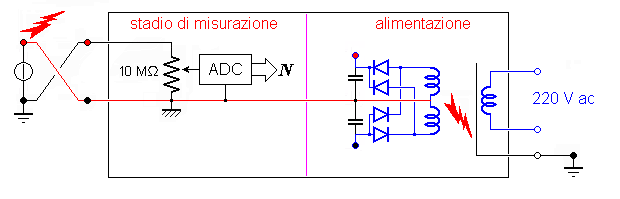
\includegraphics[scale = 1]{Misura verso terra polo caldo su polo freddo.png}
\end{figure}

Come si nota dalla riga rossa che collega polo caldo del generatore di tensione, polo freddo dello strumento di misura, 
massa dello stadio di misurazione e massa dovuto alla posizione a metà del secondario nello stadio di alimentazione, 
ci può essere una scarica di corrente molto elevata perchè il riferimento, che dovrebbe essere a 0 V, è uguale alla tensione del polo caldo del generatore di tensione. \newline 

Grazie allo schermo elettrostatico (riga nera che divide primario e secondario nello stadio di alimentazione) in teoria l'operatore che svolge la misura, e che quindi è a contatto sia con i poli del generatore di tensione sia ai poli dello strumento di misura, 
dovrebbe essere tranquillo perchè lo schermo elettrostatico permette di dividere primario e secondario dello stadio di alimentazione dello strumento. \newline 

Ma, anche se la misura viene svolta in modo corretto come nel seguente caso: 

\begin{figure}[h]
    \centering
    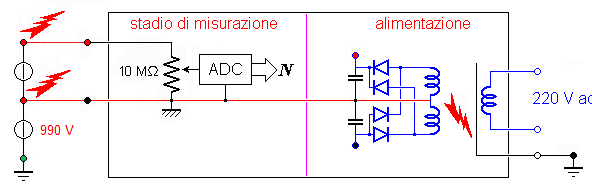
\includegraphics[scale = 1]{Misura verso terra corretta ma con tensione elevata.png}
\end{figure}


il polo freddo dello strumento di misura, che idealmente dovrebbe essere uguale a 0, assume la tensione del polo caldo del secondo generatore di tensione, 
che, in questo esempio, ha una tensione molto elevata di 900 V e ci sono le stesse problematiche dovuto ad una non corretta misurazione. \newline 

\newpage 

Per questi motivi, specialmente sopratutto riguardo alla costruzione fisica dello schermo elettrostatico, 
negli strumenti da banco possiamo trovare la seguente dicitura: 

\begin{figure}[h]
    \centering
    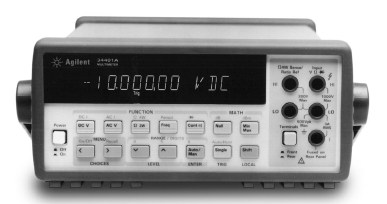
\includegraphics[scale = 1]{multimetro da banco.png}
    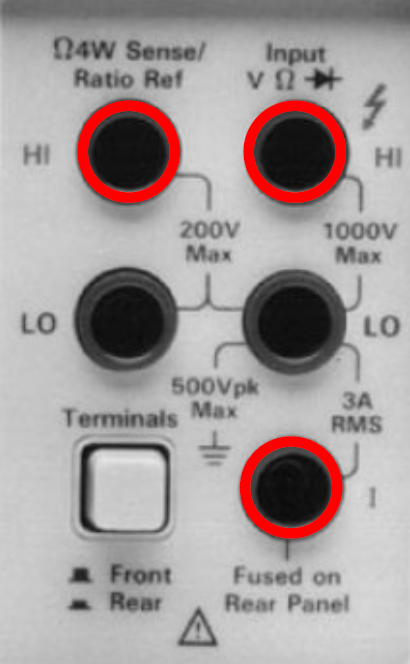
\includegraphics[scale = 0.5]{pannello bocchette multimetro da banco.PNG}
\end{figure}

Questo strumento misura massimo 1000 V ma con massimo 500 V di picco nel morsetto freddo 
(scrittura 500 $V_{pk}$ MAX). \newline 

Per evitare questi problemi, se bisogna svolgere una misura verso terra, si predilige di non utilizzare un voltmetro da banco collegato alla rete di distribuzione, 
bensì un tester collegato a batteria come il mitico Fluke 112: 

\begin{figure}[h]
    \centering
    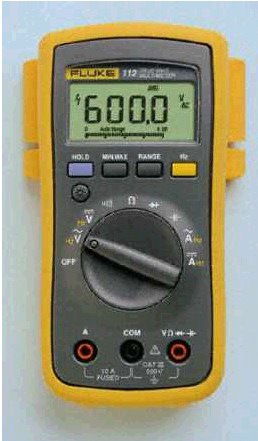
\includegraphics[scale = 0.5]{Fluke 112.png}
    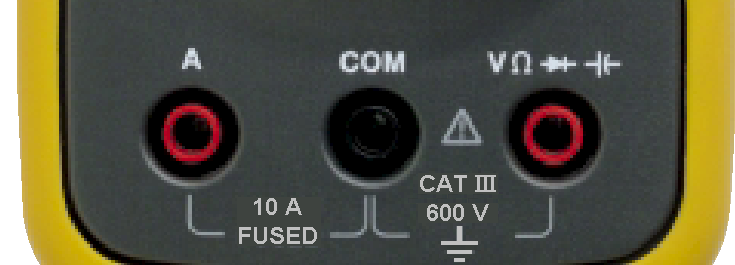
\includegraphics[scale = 0.5]{pannello bocchette tester Fluke 112.png}
\end{figure}

\newpage 